% Pipeline diagram for the T-DMB end-to-end receiver paper.
% Drop-in TikZ block: usepackage{tikz} in main.tex.
\usetikzlibrary{positioning,arrows.meta,shapes.geometric,calc}

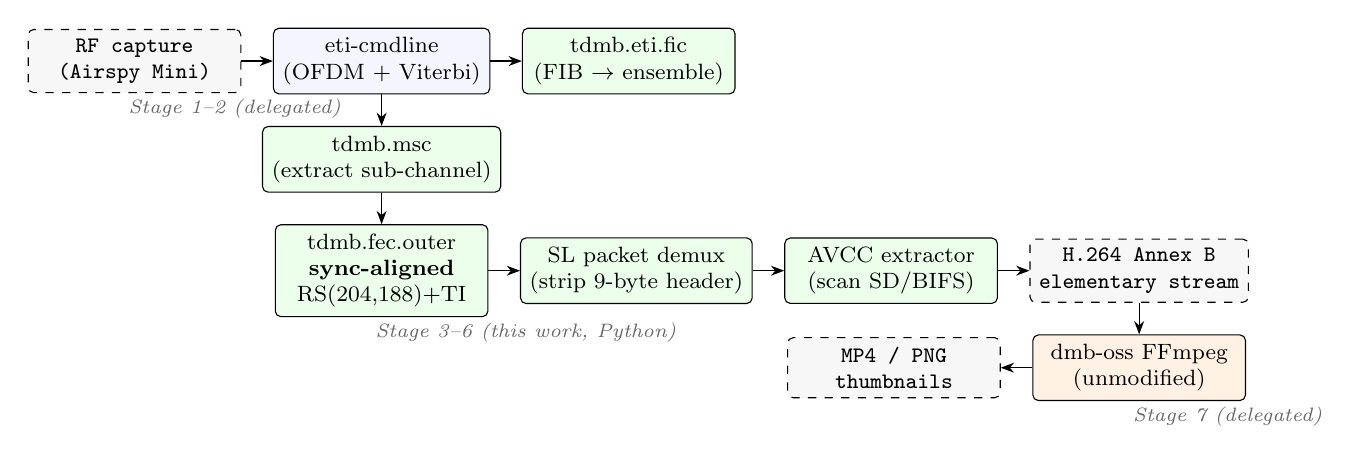
\begin{tikzpicture}[
    >=Stealth,
    node distance=4mm and 4mm,
    every node/.style={font=\footnotesize},
    stage/.style={draw, rounded corners=2pt, minimum height=8mm,
                  minimum width=27mm, align=center, fill=blue!4},
    py/.style   ={draw, rounded corners=2pt, minimum height=8mm,
                  minimum width=27mm, align=center, fill=green!8},
    ext/.style  ={draw, rounded corners=2pt, minimum height=8mm,
                  minimum width=27mm, align=center, fill=orange!10},
    io/.style   ={draw, dashed, rounded corners=2pt, minimum height=7mm,
                  minimum width=27mm, align=center, fill=black!3,
                  font=\footnotesize\ttfamily},
]

\node[io]                          (rf)    {RF capture\\(Airspy Mini)};
\node[stage, right=of rf]          (eti)   {eti-cmdline\\(OFDM + Viterbi)};
\node[py, right=of eti]            (fic)   {tdmb.eti.fic\\(FIB $\to$ ensemble)};
\node[py, below=of eti]            (msc)   {tdmb.msc\\(extract sub-channel)};
\node[py, below=of msc]            (outer) {tdmb.fec.outer\\\textbf{sync-aligned}\\RS(204,188)+TI};
\node[py, right=of outer]          (sl)    {SL packet demux\\(strip 9-byte header)};
\node[py, right=of sl]             (avcc)  {AVCC extractor\\(scan SD/BIFS)};
\node[io, right=of avcc]           (h264)  {H.264 Annex B\\elementary stream};
\node[ext, below=of h264]          (ff)    {dmb-oss FFmpeg\\(unmodified)};
\node[io, left=of ff]              (mp4)   {MP4 / PNG\\thumbnails};

\draw[->] (rf)    -- (eti);
\draw[->] (eti)   -- (fic);
\draw[->] (eti)   -- (msc);
\draw[->] (msc)   -- (outer);
\draw[->] (outer) -- (sl);
\draw[->] (sl)    -- (avcc);
\draw[->] (avcc)  -- (h264);
\draw[->] (h264)  -- (ff);
\draw[->] (ff)    -- (mp4);

\node[font=\scriptsize, anchor=west, text=black!60] at ($(rf.south)+(-2mm,-2mm)$)
      {\textit{Stage 1--2 (delegated)}};
\node[font=\scriptsize, anchor=west, text=black!60] at ($(outer.south)+(-2mm,-2mm)$)
      {\textit{Stage 3--6 (this work, Python)}};
\node[font=\scriptsize, anchor=west, text=black!60] at ($(ff.south)+(-2mm,-2mm)$)
      {\textit{Stage 7 (delegated)}};

\end{tikzpicture}
